%! TeX root = ../main.tex

\chapter{Models and formalism}%
\label{ch:models-and-formalism}

\section{Bethe lattice}%
\label{sec:bethe-lattice}

In solid-states physics we study crystals in which atoms are periodically arranged in a lattice.
Given a set of basis vectors $\{\vec{a}_i\}$,
the lattice is periodic for all translations
\begin{equation}
    \vec{R} = \sum_i n_i \vec{a}_i
\end{equation}
for any integer $n_i \in \mathbb{Z}$.

In this work however,
we look at the Bethe lattice which is only characterized by a single quantity:
the coordination number $z$.
It is an infinite graph where each vertex is connected to $z$ neighbors\footnote{
    It is a lattice in the sense that a translation shifts the root node which is set arbitrarily.
}.
A sketch for $z=3$ is given in \zcref{subfig:bethe-lattice}:
We choose the black vertex in the center as the root node.
It is connected to three nodes (marked in blue) which in turn are also connected
to three nodes (each blue node is connected to the original black node and two red nodes).
This scheme is then infinitely repeated for each site.

We can then model electron movement as hopping from a given site to
one of the $z$ neighbors.
If we assume that hopping to each nearest neighbor is equally likely and assign it the probability $p^*$,
the total probability of movement is $p = zp^*$.
In the limit of infinite connectivity $z\to\infty$ (infinite dimensions) this will diverge,
necessitating a renormalization.
Thus, the probability is rescaled as $p^* \to p^*/z$ such that
the total probability $p$ stays finite.
Instead of working with a hopping probability,
we instead introduce the hopping amplitude $t^* = t/\sqrt{z}$~\cite{Held2007}.
Such a hopping process between neighboring sites is sketched in \zcref{subfig:bethe-lattice}.

For the Bethe lattice, the density of states (DOS) for $z\to\infty$ reads
\begin{equation}
    \rho(\omega) = \frac{1}{2\muppi t^2} \sqrt{\omega^2 - 4t^2},
\end{equation}
with bandwidth $W=4t$.
This expression\footnote{
    This distribution is also known as the Wigner semicircle distribution
    which is the eigenvalue distribution of random matrices.
    They are related to the DOS in as much as a random walk on the Bethe lattice.
    As the graph has no closed loops,
    a particle must necessarily take the same path back to return to its origin.
    Further information can be found in the literature under \emph{random matrix theory}.
}
is commonly written using the half-bandwidth $D = W/2 = 2t$:
\begin{equation}
    \rho(\omega) = \frac{2}{\muppi D^2} \sqrt{\omega^2 - D^2},
    \label{eq:dos-semicircle}
\end{equation}
which is shown in \zcref{subfig:bethe-density}.

\begin{figure}[ht]
    \centering
    \begin{subfigure}{0.45\textwidth}
        \centering
        %! TeX root = ../../main.tex

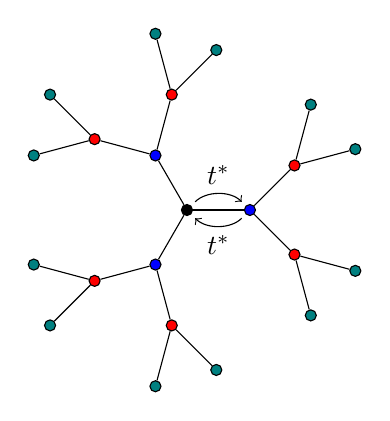
\begin{tikzpicture}
    [
        level distance=8mm,
        site/.style={
                circle,
                inner sep=0pt,
                minimum size=4pt,
                draw=black,
                fill=#1,
            },
    ]

    % Bethe lattice with connectivity z=3 using built-in tree functionality
    % angles for each distance are: 60, 45, 30
    \node [site=black] (s0) {} % root
    child [grow=0] % right
        {
            node [site=blue] (s1) {}
            child [grow=45]
                {
                    node [site=red] {}
                    child [grow=15]
                        {
                            node [site=teal] {}
                        }
                    child [grow=75]
                        {
                            node [site=teal] {}
                        }
                }
            child [grow=-45]
                {
                    node [site=red] {}
                    child [grow=-15]
                        {
                            node [site=teal] {}
                        }
                    child [grow=-75]
                        {
                            node [site=teal] {}
                        }
                }
        }
    child [grow=120] % top left
        {
            node [site=blue] {}
            child [grow=75]
                {
                    node [site=red] {}
                    child [grow=45]
                        {
                            node [site=teal] {}
                        }
                    child [grow=105]
                        {
                            node [site=teal] {}
                        }
                }
            child [grow=165]
                {
                    node [site=red] {}
                    child [grow=135]
                        {
                            node [site=teal] {}
                        }
                    child [grow=195]
                        {
                            node [site=teal] {}
                        }
                }
        }
    child [grow=240] % bottom right
        {
            node [site=blue] {}
            child [grow=195]
                {
                    node [site=red] {}
                    child [grow=165]
                        {
                            node [site=teal] {}
                        }
                    child [grow=225]
                        {
                            node [site=teal] {}
                        }
                }
            child [grow=285]
                {
                    node [site=red] {}
                    child [grow=255]
                        {
                            node [site=teal] {}
                        }
                    child [grow=315]
                        {
                            node [site=teal] {}
                        }
                }
        };

    % hopping
    \draw [->,shorten <=2pt, shorten >=2pt] (s0.north east) to [bend left=45] node[midway, above] {$t^*$} (s1.north west);
    \draw [<-,shorten <=2pt, shorten >=2pt] (s0.south east) to [bend right=45] node[midway, below] {$t^*$} (s1.south west);
\end{tikzpicture}

        \caption{}%
        \label{subfig:bethe-lattice}
    \end{subfigure}
    \begin{subfigure}{0.45\textwidth}
        \centering
        %! TeX root = ../../main.tex

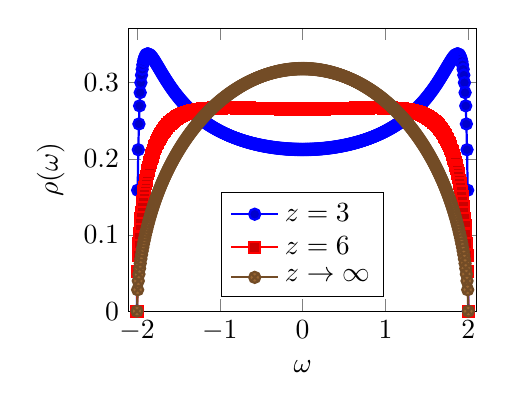
\begin{tikzpicture}
    \begin{axis}
        [
            width=6cm,
            xlabel=$\omega$,
            ylabel=$\rho(\omega)$,
            xmin=-2.1,
            xmax=2.1,
            ymin=0,
            every axis plot/.append style=
                {
                    thick,
                    domain=-2:2,
                    samples=513, % 2^n + 1 to ensure inclusion of last point
                },
            legend cell align=left,
            legend entries={
                    $z=3$,
                    $z=6$,
                    $z\rightarrow\infty$,
                },
            legend style={
                    at={(0.5, 0.05)},
                    anchor=south,
                },
        ]

        \addplot {1/(2*pi) * sqrt(4 - x^2) / (3/(3-1) - x^2/3}; % z=3
        \addplot {1/(2*pi) * sqrt(4 - x^2) / (6/(6-1) - x^2/6}; % z=6
        \addplot {1/(2*pi) * sqrt(4 - x^2)}; % z\to\infty
    \end{axis}
\end{tikzpicture}

        \caption{}%
        \label{subfig:bethe-density}
    \end{subfigure}
    \caption{
        \subref{subfig:bethe-lattice}
        Bethe lattice with coordination number $z=3$ and hopping amplitude $t^*$.
        \subref{subfig:bethe-density}
        DOS in infinite dimensions for $D=1$.
        \fe{TODO: align sub figures?} %TODO: align subfigures? % chktex 13
    }
\end{figure}

\section{Hubbard model}%
\label{sec:hubbard-model}

Although we do not explicitly calculate properties of the system through the
Hubbard model~\cite{Hubbard1997},
we nevertheless want to mention it briefly due to its importance in DMFT\@.
Denoting the creator of site $i$ and spin $\sigma\in\{\uparrow,\downarrow\}$
as $d^\dag_{i\sigma}$ and respective annihilator as $d_{i\sigma}$ its Hamiltonian\footnote{
    In this work we look at the SU(2) symmetric model % chktex 36
    which means that quantities (e.g.,\ on-site energies) are spin-independent.
    Thus, we omit the spin index.
}
reads
\begin{equation}
    H
    =
    -t\sum_{\langle i j\rangle\sigma}
    (d^\dag_{i\sigma} d^{\pdag}_{j\sigma} + d^\dag_{j\sigma} d^{\pdag}_{i\sigma})
    +
    U\sum_i n_{i\uparrow} n_{i\downarrow}
    +
    (\epsilon - \mu)\sum_{i\sigma} n_{i\sigma},
    \label{eq:H-Hubbard}
\end{equation}
with a sketch given in \zcref{fig:hubbard-model}.
\begin{figure}[ht]
    \centering
    %! TeX root = ../../main.tex
% chktex-file 8

\def\nsites{3}
\def\len{3mm}
\def\wdth{3mm}
\def\lwdth{0.75mm}
\def\spinsep{0.1}

\newcommand\nup[2]
{
    \draw [red, {Latex[length=\len, width=\wdth]}-, line width=\lwdth]
    ({#2*2}, {0.6-#1*2}) -- ({#2*2}, {-0.6-#1*2});
}

\newcommand\ndn[2]
{
\draw [blue, -{Latex[length=\len, width=\wdth]}, line width=\lwdth]
({#2*2}, {0.6-#1*2}) -- ({#2*2}, {-0.6-#1*2});
}

\newcommand\nupdn[2]
{
\draw [red, {Latex[length=\len, width=\wdth]}-, line width=\lwdth]
({#2*2-\spinsep}, {0.6-#1*2}) -- ({#2*2-\spinsep}, {-0.6-#1*2});
\draw [blue, -{Latex[length=\len, width=\wdth]}, line width=\lwdth]
({#2*2+\spinsep},{0.6-#1*2}) -- ({#2*2+\spinsep},{-0.6-#1*2});
\node at ({#2*2+0.5},{-#1*2+0.5}) {$U$};
}

\newcommand\hoppingdown[2]{
    \draw [->, thick]
    ({#2*2-0.4}, {-0.4-#1*2}) to [bend right=30] node[midway, left] {$t$} ({#2*2-0.4}, {-1.6-#1*2});
}

\newcommand\hoppingright[2]{
    \draw [->, thick]
    ({#2*2+0.4}, {0.4-#1*2}) to [bend left=30] node[midway, above] {$t$} ({#2*2+1.6}, {0.4-#1*2});
}

\begin{tikzpicture}
    [
        node distance=10mm,
        inner sep=1mm,
        minimum size=5mm,
        site/.style={rectangle,draw=black,very thick,fill=gray!20},
    ]
    % grid
    \draw [dashed] (1,-1) grid[step=20mm] (2*\nsites+1,-2*\nsites-1);
    % sites
    \foreach \x in {1,...,\nsites}
        {
            \foreach \y in {1,...,\nsites}
                {
                    % \node [site, label=\x\y] at (2*\x,-2*\y) (s\x\y) {};
                    \node [site] at (2*\x,-2*\y) (s\x\y) {};
                }
        }
    % add electrons
    \nup{1}{1}
    \ndn{1}{2}
    \nupdn{1}{3}
    \ndn{2}{3}
    \nup{3}{1}
    \nupdn{3}{2}
    \hoppingdown{1}{1}
    \hoppingright{1}{1}
\end{tikzpicture}

    \caption{
        Hubbard model for a 2D square lattice.
        $t$ denotes hopping between neighboring sites
        and $U$ describes the Coulomb repulsion on a doubly occupied site.
    }%
    \label{fig:hubbard-model}
\end{figure}
Each site can be occupied by up to two electrons.
The first term describes the kinetics of the system:
Electrons can hop between nearest-neighbors $\langle i j\rangle$
with the hopping amplitude $t$.
If two electrons are on the same site, they are repulsed by the local Coulomb interaction $U$
expressed by the second term (occupation $n_{i\sigma} = d^\dag_{i\sigma} d^{\pdag}_{i\sigma}$).
The last term describes the on-site energy $\epsilon$ and
chemical potential $\mu$ which control the average occupation per site.
In this work we look at the half-filled system $\epsilon=0$,  $\mu=U/2$
with average occupation $\expval{n} = 1$.


Although the model Hamiltonian looks simple at first glance,
no analytical solution exists for the general case.
The problem is that the kinetic part is diagonal in momentum space,
while the Coulomb interaction is diagonal in real space.

\section{Anderson impurity model}%
\label{sec:anderson-impurity-model}

Instead of having a repulsion $U$ on each site,
we can create a model in which only one site is correlated
(called \emph{impurity site} or just \emph{impurity})
and embedded in a non-interacting bath.
This is called the Anderson impurity model~\cite{Anderson1961}
and its Hamiltonian can be written as
\begin{equation}
    H = H_\mathrm{imp} + H_\mathrm{bath} + H_\mathrm{imp - bath}.
    \label{eq:H-Anderson}
\end{equation}
The impurity can be further split into a non-interacting and interacting part
using the occupation operator $n_\sigma = d^\dag_\sigma d^{\pdag}_\sigma$
\begin{align}
    H_{\mathrm{imp},0} & = (\epsilon - \mu) \sum_\sigma n_\sigma \\
    H_\mathrm{int}     & = U n_\uparrow n_\downarrow,
    \label{eq:H-Anderson-interaction}
\end{align}
which has overlapping terms with \zcref{eq:H-Hubbard}.
For the bath we define the annihilator $b_{k\sigma}$ and energy $\epsilon_k$,
allowing us to write
\begin{equation}
    H_\mathrm{bath} = \sum_{k\sigma} \epsilon_k b^\dag_{k\sigma} b^{\pdag}_{k\sigma}.
\end{equation}
Finally, the interaction between impurity and bath is given by the hybridization strength $V_k$:
\begin{equation}
    H_\mathrm{imp - bath}
    =
    \sum_{k\sigma} \left(V^{\ps}_k d^\dag_{\pk\sigma} b^{\pdag}_{k\sigma}
    + V_k^* b^\dag_{k\sigma} d^{\pdag}_{\pk\sigma} \right)
\end{equation}
A graphical representation of the Hamiltonian in \zcref{eq:H-Anderson} is given
in \zcref{fig:AIM-geometry-star}:
each bath site has a given filling
and electrons from each bath site can hop in and out of the impurity.
\begin{figure}[ht]
    \centering
    %! TeX root = ../../main.tex

\begin{tikzpicture}
    [
        node distance=2mm,
    ]
    % draw sites
    \foreach \i [remember=\i as \lasti, evaluate=\i as \filling using -0.1*\i+0.9] in {1,...,7}
        {
            \ifnum\i=1
                \node [bath={\filling}, label=right:$l_\i$] (l\i) {};
            \else
                \node [bath={\filling}, label=right:$l_\i$] (l\i) [above=of l\lasti] {};
            \fi
        }
    \node [impurity={0.5}, label=left:$i$] (impurity) [left=5mm of l4] {};

    % connect sites
    \foreach \i in {1,...,7}
        {
            \draw (impurity.east) to [out=0,in=180,looseness=0.3] (l\i.west);
        }
\end{tikzpicture}

    \caption{
        Sketch of an Anderson impurity model.
        Impurity (square) interacting with bath sites (circles).
        Site occupation is indicated by fill level,
        where a full site corresponds to double occupation.
        Furthermore, hopping between the impurity and bath sites is shown by lines.
        (adapted from~\cite{Lu2019}).
    }%
    \label{fig:AIM-geometry-star}
\end{figure}
The last two terms of \zcref{eq:H-Anderson} are commonly combined into the
\emph{hybridization function}
\begin{equation}
    \Delta_\omega = \sum_{k} \frac{|V_k|^2}{\omega + \mi0^+ - \epsilon_k}.
\end{equation}

\section{Green's function and correlators}%
\label{sec:greens-function-correlators}

The retarded Green's function is defined as
\begin{equation}
    G(t) = -\mi \Theta(t) \expval{\acomm{d^{\pdag}_{i\sigma}(t)}{d^\dag_{i\sigma}}},
\end{equation}
with the step function $\Theta$ and anticommutator $\acomm{\cdot}{\cdot}$.
$d_{i\sigma}(t) = \me^{\mi H t} d_{i\sigma} \me^{-\mi H t}$ is given
in the Heisenberg picture\footnote{
    In this work we look at time-independent Hamiltonians.
    Thus, we can set our time origin arbitrarily and
    our time evolution operator is given as $U(t, 0) = \me^{-\mi H t}$
    which evolves the system from $0$ to $t$.
    Otherwise, one needs to use a general time evolution $U(t, t_0)$
}.
At zero temperature $T=0$, the expectation value is evaluated on the ground state
$\expval{\,\cdot\,} = \sandwich{\psi_0}{\,\cdot\,}{\psi_0}$ only.
This function consists of two terms which can be interpreted as
the propagation of a particle or hole respectively,
e.g., at time $0$ a particle is added at site $i$ with spin $\sigma$.
The system then evolves as dictated by the Hamiltonian.
At a later time $t$ the particle is then removed from the same site.
The Green's function can therefore be interpreted as the probability amplitude
of a particle returning to its origin at time $t$.

This method can be generalized for two arbitrary fermionic operators $A, B$ defining
a \emph{correlation function} or just \emph{correlator}
\begin{equation}
    C(t) = -\mi \Theta(t) \expval{\acomm{A(t)}{B}}.
    \label{eq:correlator-time}
\end{equation}
Following the notation of~\cite{Bulla1998,Kugler2022},
we will denote the Fourier transform\footnote{
    As our Hamiltonian is hermitian, its eigenvalues (poles) lie on the real axis.
    This means that the correlator is analytic in the upper and lower complex plane
    and allows us to approach it from above $\omega + \mi 0^+$ (retarded)
    or below $\omega - \mi 0^+$ (advanced).
    Using different approaches for $\omega\gtrless0$ gives rise to the causal and anti-causal correlator.
}
as
\begin{equation}
    C_\omega
    \coloneq
    \lim_{\delta\to0^+}
    \int_{-\infty}^\infty\! \md t\> \me^{\mi (\omega + \mi\delta) t} C(t)
    \eqcolon
    \dangle{A}{B}{\omega}.
\end{equation}
Given the ground state energy $E_0$
and splitting this expression into two components $C_\omega = C^+_\omega + C^-_\omega$\footnote{
    $C^+_\omega$ has poles on the positive real axis
    while $C^-_\omega$ has poles on the negative real axis.
}
gives
\begin{subequations}
    \begin{align}
        C^+_\omega
         & =
        \expval*{A \frac{1}{\omega + \mi0^+ - (H - E_0)} B}, \\
        C^-_\omega
         & =
        \expval*{B \frac{1}{\omega + \mi0^+ + (H - E_0)} A}.
    \end{align}
    \label{eq:correlator-frequency} % chktex 24
\end{subequations}
A detailed derivation is available in \zcref{app:fourier-transform}.
As we are only interested in energies relative to the ground state,
we can absorb it into our Hamiltonian
\begin{equation}
    H \to H - E_0
    \label{eq:Hamiltonian-shift}
\end{equation}
such that all eigenvalues are non-negative: $H\ket{n} = E_n\ket{n}$ with $E_n \ge 0$.
E.g., for the Green's function on the positive real axis we can write
\begin{equation}
    G^+_\omega
    =
    \sum_n
    \frac{\sandwich{\psi_0}{d^{\pdag}_{i\sigma}}{n}\sandwich{n}{d^\dag_{i\sigma}}{\psi_0}}{\omega + \mi0^+ - E_n}
    =
    \sum_n
    \frac{|\sandwich{n}{d^\dag_{i\sigma}}{\psi_0}|^2}{\omega + \mi0^+ - E_n}.
\end{equation}

\subsection{Spectral function}

\begin{figure}[ht]
    \centering
    %! TeX root = ../../main.tex

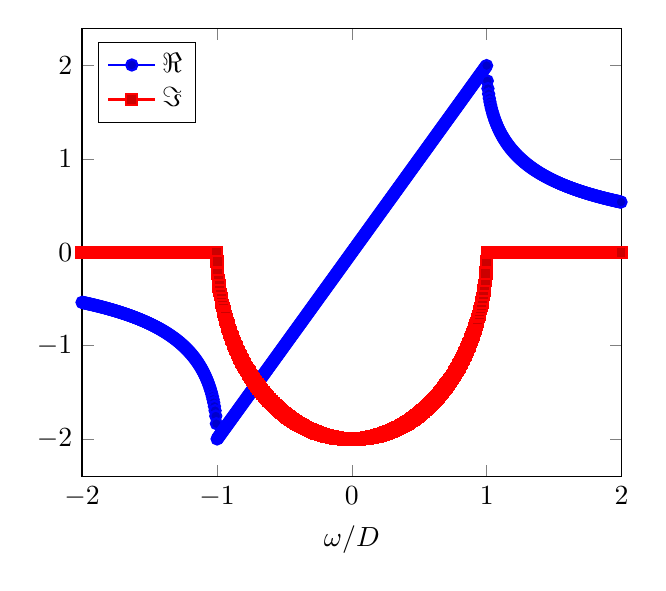
\begin{tikzpicture}
    \begin{axis}[
            xlabel=$\omega/D$,
            xmin=-2,
            xmax=2,
            every axis plot/.append style={
                    thick,
                    domain=-2:2,
                    samples=800,
                },
            legend entries={
                    $\Re$,
                    $\Im$,
                },
            legend pos=north west,
        ]

        \addplot {
            x < -1 ?
            % (-\infty, -D)
            2 * (x + sqrt(x^2 - 1))
            :
            (
            x < 1 ?
            % [-D, D)
            2 *x
            :
            % [D, \infty)
            2 * (x - sqrt(x^2 - 1))
            )
        };
        \addplot {abs(x) < 1 ? -2 * sqrt(1 - x^2) : 0};
    \end{axis}
\end{tikzpicture}

    \caption{
        Real and imaginary part of the Green's function of the
        Bethe lattice in infinite dimensions.
    }%
    \label{fig:bethe-greens-function}
\end{figure}
Given our Green's function,
we can split it up into a real and imaginary part.
Taking the latter and rescaling it allows us to define the spectral function
\begin{equation}
    A_\omega \coloneq -\frac{1}{\muppi}\Im G_\omega,
\end{equation}
which is generalized to the \emph{spectral part} of $C$
\begin{equation}
    A_\omega \coloneq -\frac{1}{\muppi}\Im C_\omega.
\end{equation}
As our correlator is analytic in the upper complex plane,
the real and imaginary part are not independent
but related by Kramers-Kronig transformations (Hilbert transform)
\begin{subequations}
    \begin{align}
        \Re C_\omega
         & =
        - \frac{1}{\muppi} \mathcal{P}\! \int_{-\infty}^\infty\! \md\omega'
        \frac{\Im C_{\omega'}}{\omega - \omega'}
        \label{eq:kramers-kronig-real} \\
        \Im C_\omega
         & =
        \phantom{-} \frac{1}{\muppi} \mathcal{P}\! \int_{-\infty}^\infty\! \md\omega'
        \frac{\Re C_{\omega'}}{\omega - \omega'}.
        \label{eq:kramers-kronig-imag}
    \end{align}
\end{subequations}
Thus, using our non-interacting density of the Bethe lattice (\zcref{eq:dos-semicircle})
as a spectrum,
we can calculate the corresponding real part.
This allows us to create a non-interacting Green's function~\cite{Economou2006}
(labeled with a subscript $0$)
\begin{equation}
    G_{0,\omega}
    =
    \frac{2}{D^2} \left(\omega - \sgn(\omega) \sqrt{\omega^2 - D^2}\right),
\end{equation}
shown in \zcref{fig:bethe-greens-function}.
The signum function at zero is defined as $\sgn(0^\pm) = \pm 1$.
As the complex square root has a branch cut,
the imaginary part is taken to be positive.

Due to the self-similarity of the Bethe lattice,
its hybridization function is just a rescaled Green's function
\begin{equation}
    \Delta_\omega = \frac{D^2}{4} G_\omega.
\end{equation}

\subsection{Moments}%
\label{sec:moments}

The moments of a correlator~\cite{Lu2014,Kugler2022,Potthoff1997} are defined as
\begin{equation}
    C^{(n)}
    =
    -\frac{1}{\muppi} \int_{-\infty}^\infty\! \md\omega\> \omega^n \Im C_\omega
    =
    \int_{-\infty}^\infty\! \md\omega\> \omega^n A_\omega,
\end{equation}
allowing us to write a high-frequency expansion
\begin{equation}
    C_\omega = \sum_{n=0}^\infty \frac{C^{(n)}}{\omega^{n+1}}.
    \label{eq:expansion-correlator}
\end{equation}

An alternative but equivalent approach is to use the Heisenberg equation of motion.
We define $\mathcal{L}A = [A, H]$ as the commutator of an operator $A$ with the Hamiltonian
which allows us to formulate the moments as
\begin{equation}
    C^{(n)} = \expval{\acomm{\mathcal{L}^n A}{B}},
\end{equation}
e.g., $G^{(0)} = \expval{\acomm{d^{\pdag}_{i\sigma}}{d^\dag_{i\sigma}}} = 1$
by definition of anticommutative rules for fermionic operators.
For the particle-hole symmetric system on the Bethe lattice
the first four moments of the Green's function are~\cite{Potthoff1997}
\begin{align}
    G^{(0)} & = 1,                             \\
    G^{(1)} & = 0,                             \\
    G^{(2)} & = \frac{U^2}{2} + \frac{D^2}{4}, \\
    G^{(3)} & = 0.
\end{align}
Due to symmetry $A_{-\omega} = A_\omega$ for the half-filled spectrum,
all odd moments vanish.

\section{Self-energy}%
\label{sec:self-energy}

As mentioned in the previous section,
the Green's function $G_\omega$ describes the propagation of an electron/hole in our system.
The quantity that connects these between an interacting and non-interacting system
is the so-called \emph{self-energy} defined by the Dyson equation\footnote{
    This equation can be motivated by Feynman diagrams.
}
\begin{equation}
    \Sigma_\omega = (G_{0, \omega})^{-1} - (G_\omega)^{-1}.
    \label{eq:Dyson}
\end{equation}

We can define the moments of the self-energy in the same way as correlators in \zcref{sec:moments},
allowing us to write down a high-energy expansion
\begin{equation}
    \Sigma_\omega = \sum_{n=-1}^\infty \frac{\Sigma^{(n)}}{\omega^{n+1}}.
\end{equation}
In contrast to \zcref{eq:expansion-correlator},
the self-energy contains a constant (frequency intependent) term
which is called the Hartree term $\Sigma^\mH$.
The analytic moments for half-filling are~\cite{Potthoff1997}
\begin{align}
    \Sigma^\mH   & = \frac{U}{2},   \\
    \Sigma^{(0)} & = \frac{U^4}{4}, \\
    \Sigma^{(1)} & = 0,             \\
\end{align}
with every odd moment vanishing.

Although the Dyson equation (\zcref{eq:Dyson}) is exact,
it poses an issue~\cite{Bulla1998}:
$G_{0,\omega}$ is known analytically while
$G_\omega$ can only be obtained numerically most of the time.
Thus, calculating the difference as dictated by \zcref{eq:Dyson} is prone to
catastrophic cancellation if the difference becomes very small\footnote{
    This happens around the Fermi level which is the most important region.
}.
To mitigate this,
\citeauthor{Bulla1998} calculated the self-energy using a quotient of two correlators.
In this work we go a step further by using the symmetric improved estimator
$\Sigma^\mIFG_\omega$~\cite{Kugler2022}
which will be summarized in the following:
We introduce the auxiliary operator
\begin{equation}
    q_\sigma = \comm{d_\sigma}{H_\mathrm{int}}
\end{equation}
with the interacting Hamiltonian from \zcref{eq:H-Anderson-interaction},
allowing us to calculate the Hartree term directly
\begin{equation}
    \Sigma^\mH = \expval{\acomm{q^\dag_\sigma}{d^{\pdag}_\sigma}}.
\end{equation}
We then employ a quadratic shift\footnote{
    As noted by \citeauthor{Kugler2022},
    this is especially convenient for particle-hole symmetric systems.
}
\begin{equation}
    \tilde q_\sigma = q_\sigma - \Sigma^\mH d_\sigma
    \label{eq:quadratic-shift}
\end{equation}
and obtain four correlation functions
\begin{subequations}
    \begin{alignat}{2}
        G_\omega
         & =
        \dangle{d^{\pdag}_\sigma}{d_{\sigma}^\dag}{\omega},
         &
        \qquad
        I_\omega
         & =
        \dangle{\tilde q^{\pdag}_\sigma}{\tilde q_{\sigma}^\dag}{\omega}, \\
        F^\mL_\omega
         & =
        \dangle{\tilde q^{\pdag}_\sigma}{d_{\sigma}^\dag}{\omega},
         &
        \qquad
        F^\mR_\omega
         & =
        \dangle{d^{\pdag}_\sigma}{\tilde q_{\sigma}^\dag}{\omega}.
    \end{alignat}%
    \label{eq:correlators}
\end{subequations}
The self-energy is computed as
\begin{equation}
    \Sigma^\mIFG_\omega
    =
    \Sigma^\mH + I_\omega - F^\mL_\omega (G_\omega)^{-1} F^\mR_\omega.
\end{equation}

\section{DMFT}%
\label{sec:dmft}

As mentioned in \zcref{sec:hubbard-model},
the Hubbard model has no analytical solution in arbitrary dimensions $d$.
In the limit $d\to\infty$ however, it can be solved by
dynamical mean-field theory (DMFT)~\cite{Georges1996},
which takes a single lattice site as a representative
and averages all spacial fluctuations around it, only keeping time correlations
(hence the term \emph{dynamical mean-field}).

A given Hamiltonian is solved by a self-consistency loop,
which repeatedly maps between the Hubbard model and Anderson impurity model.
Given a Hubbard Hamiltonian, we can define its local Green's function
\begin{equation}
    G_{\mloc,\omega}
    =
    \frac{1}{V_\mBZ} \int_\mBZ \md\vec{k}\> G_{\vec{k}\omega}
    \approx
    \frac{1}{V_\mBZ} \int_\mBZ \md\vec{k}\> \frac{1}{\omega + \mi0^+ + \mu - \epsilon_{\vec{k}} - \Sigma_\omega},
    \label{eq:greens-function-local}
\end{equation}
where the approximation assumes that the lattice self-energy is purely local
($\Sigma_{\vec{k}\omega} \to \Sigma_\omega$).
DMFT then enforces that this Green's function coincides with the impurity Green's function
of the corresponding Anderson impurity model: $G_{\mloc,\omega} \equiv G_\omega$.

Rearranging the Dyson equation (\zcref{eq:Dyson}) for the impurity
then gives us a non-interacting impurity
Green's function
\begin{align}
    (G_{0,\omega})^{-1}
     & =
    (G_{\mloc,\omega})^{-1} + \Sigma_\omega \\
     & =
    \omega + \mi0^+ + \mu - \epsilon - \Delta_\omega,
\end{align}
which is rewritten into terms,
containing the impurity energy $\epsilon - \mu$ and hybridization function $\Delta_\omega$.
Given these terms, we can write down the non-interacting Hamiltonian
of \zcref{eq:H-Anderson}.
After adding the interacting term of \zcref{eq:H-Anderson-interaction},
we can solve the impurity Hamiltonian
yielding us a new impurity Green's function $G_\omega$
and self-energy $\Sigma_\omega$.
Subsequently,
we use this impurity self-energy to
calculate a new lattice Green's function using \zcref{eq:greens-function-local},
closing our self-consistency loop.

For the special case of a lattice in infinite dimensions,
one can skip the calculation of the lattice Green's function
and directly update the hybridization~\cite{Lu2014}:
\begin{equation}
    \Delta_\omega = \Delta_{0}(\omega + \mu - \mu_0 - \Sigma_\omega),
\end{equation}
with a derivation given in \zcref{app:dmft-simplification}.
